% 2011 年天津卷理科第 6 题：△ABC 中 D 是边 AC 上的点，连 BD。
% 来源 PDF：普通高考/2011/2011天津理.pdf，SHA-256 4d77f7437f1f7191d1fd3cd766c7c3014859dec8fdd7a4d8f4bca348c0ef06e5。
% 原页：第 1 页（A3 三栏）第 1 栏下部，书页码 705。
% 重绘依据：照原页 B 在上、A 在左下、C 在右下，D 落在 AC 上靠左约四成处，连 BD；
%   AB=AD（故 D 取使 AD=AB 的位置），不按比例。
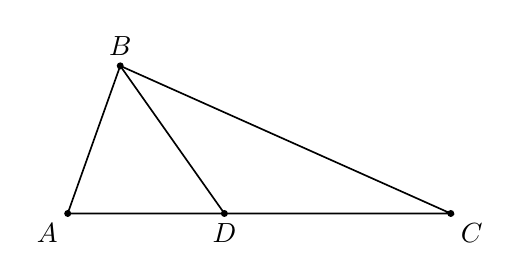
\begin{tikzpicture}[scale=1.15, >=stealth, semithick]
  \coordinate (A) at (0,0);
  \coordinate (B) at (0.58,1.63);
  \coordinate (C) at (4.23,0);
  \coordinate (D) at (1.73,0);
  \draw (A) -- (B) -- (C) -- cycle;
  \draw (B) -- (D);
  \fill (A) circle (1.1pt);
  \fill (B) circle (1.1pt);
  \fill (C) circle (1.1pt);
  \fill (D) circle (1.1pt);
  \node at (A) [below left] {$A$};
  \node at (B) [above] {$B$};
  \node at (C) [below right] {$C$};
  \node at (D) [below] {$D$};
\end{tikzpicture}
